\chapter{Poroelastic natural coatings}

\section{Biomimetics of poroelastic coatings}

Usually when someone is asked to imagine some "rapid" object as an airplane, a boat or a car, the common sense lead us to think about it as the smoothest as possible and most of the time shiny.
But if we look around us the nature seems not to agree with the previous statement.
In fact most of the surfaces in nature are not smooth at all, they present almost always some kind more or less regular arrangement of discontinuities at various length scales.
Since Nature have had a very large time-span to optimize this kind of surfaces we can be very certain that they are the best possible option.
One should pinpoint that the non smoothness of these surfaces can be connected to some other biological functions rather than pure fluid dynamic performance, and of course it can be the case.


With that in mind we want to show to the reader some of the most notably examples of "natural" aerodynamically surfaces.

Probably the most notable example is the shark skin, in figure \ref{fig:shark} a segment of the skin is depicted as if appears to be under the microscope.

\begin{figure}[h]
	\centering
	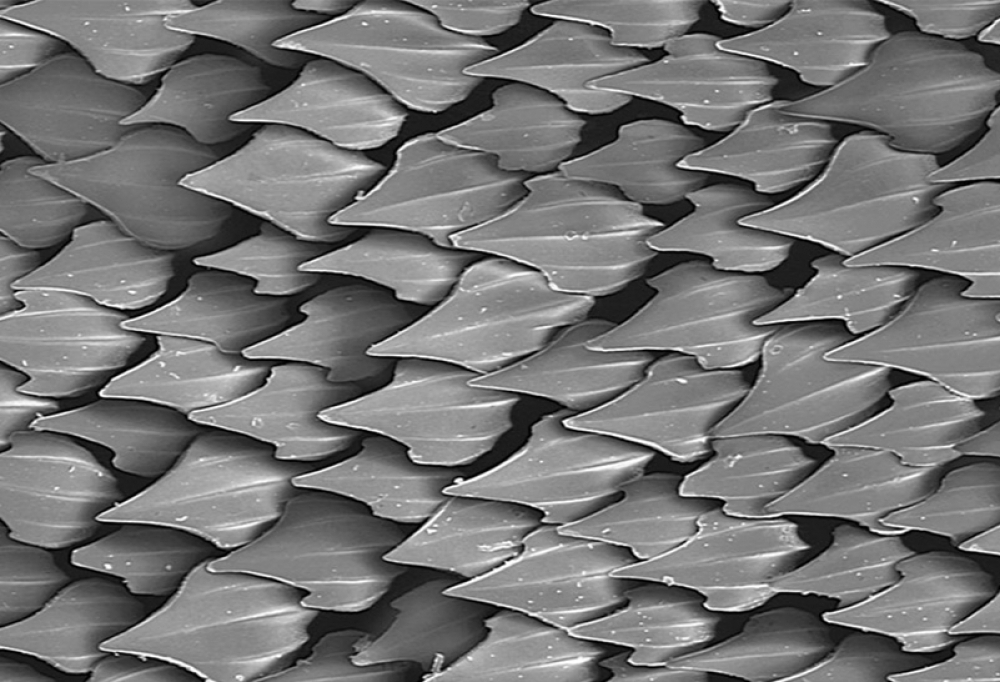
\includegraphics[width=0.6\linewidth]{chapter_1/shark}
	\caption{Microscope enlarged picture of the shark skin.}
	\label{fig:shark}
\end{figure}

The enlargement show that the surface is made up by a series of overlapped denticles, and experiment shows that they can move and interact with the flow.

The shark technology has somehow been applied by Speedo$^{\circledR}$ in their famous swimming suits, that had break multiples world records.
But it seems that this controversial swimmers performance came more on the compressed and streamlined body shape than from the surface texture itself.
In fact during the years this texture material has been publicized to be like synthetic shark skin but \cite{Oeffner785} has shown that the texture is somehow different from the shark dermal structure.
They have also performed some swimming experiment with a flat plate with different surfaces and they have found no significant speed enhancement with the swimsuit surfaces; but the measurements with the shark skin on the contrary give an appreciable improvement in the performance.


Poroelastic surfaces find also applications in aeroacoustics, in fact the owl is well known for its particularly silent flight, in the high frequency spectrum.
This characteristic is crucial for the owl in order to be able to capture his preys.
Obviously it has inspired the scientific community to study the feathers configuration and their shape.

\begin{figure}[h]
	\centering
	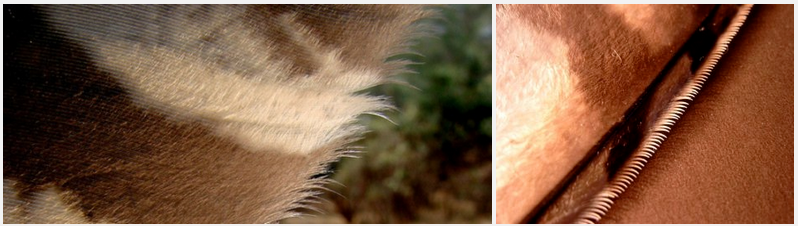
\includegraphics[width=0.8\linewidth]{chapter_1/howl}
	\caption{Feathers in owl's wing: trailing edge (left), leading edge (right). The difference in shape, and mechanical properties as rigidity, between the leading and trailing edge is a consequence of the different flow regimes in the wing.}
	\label{fig:owl}
\end{figure}
 
Multiple authors show promising result in characterizing the acoustic properties of the owl skin and their physical mechanism.
In particular \cite{lilley1998} present three main characteristic of the owl that can suppress its airborne noise: the feathers leading edge shaped like a comb, the feathers trailing edge that form a fringe and the presence of multiple "filaments" in the bottom surface of the wing and on its legs.
in the same work he also present some experimental and empirical evidence on the aeroacoustics mechanism behind the three elements above.

Another examples of work in the field of owls acoustic is the one by \cite{jaworski2013aerodynamic} in which the authors study the acoustic scattering problem of a poroelastic half-plane hit by an incident plane wave.
This configuration has been used as an analogy with the owl wing, it try to explain how the properties of this surface can suppress the noise.
They conclude that the combined effects of elasticity and porosity can produce the weakest edge noise amplification.

Recent computational simulation made by \cite{rao2017owl} confirm that the leading edge shape of the feathers truly suppress noise and enhance the lift generation for angles of attack grater then $15^{\circ}$.


Bioinspired aerodynamic surfaces include another peculiar example in the butterflies wings.
In figure \ref{fig:butterfly} the surface of a "Peacock butterfly" is enlarged in order to show the multiple scales involved; the wing structure present firstly as overlapped scales similar to the shark, but looking closely we can observe that the singles scales have a complicated permeable structure.

\begin{figure}[h]
	\centering
	\begin{subfigure}[b]{0.3\textwidth}
		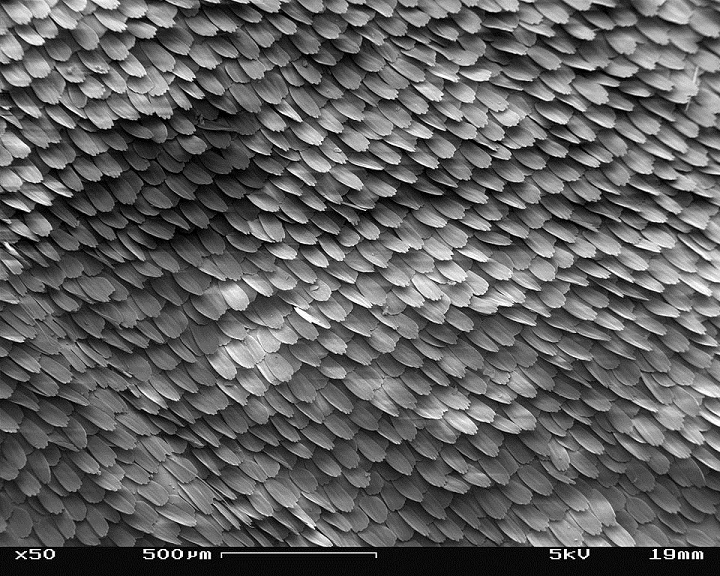
\includegraphics[width=\textwidth]{chapter_1/butterfly}
		\caption{Magnification 50x}
		\label{fig:b50}
	\end{subfigure}
	~ %add desired spacing between images, e. g. ~, \quad, \qquad, \hfill etc. 
	%(or a blank line to force the subfigure onto a new line)
	\begin{subfigure}[b]{0.3\textwidth}
		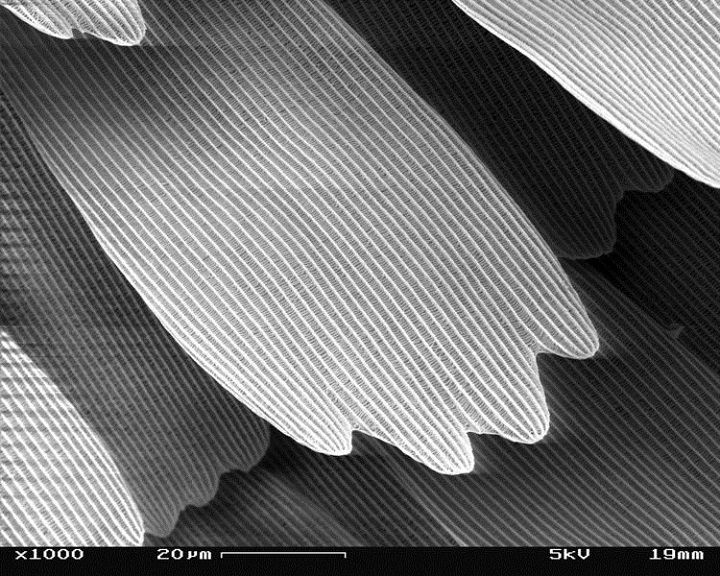
\includegraphics[width=\textwidth]{chapter_1/butterfly2}
		\caption{Magnification 1000x}
		\label{fig:b1000}
	\end{subfigure}
	\begin{subfigure}[b]{0.3\textwidth}
		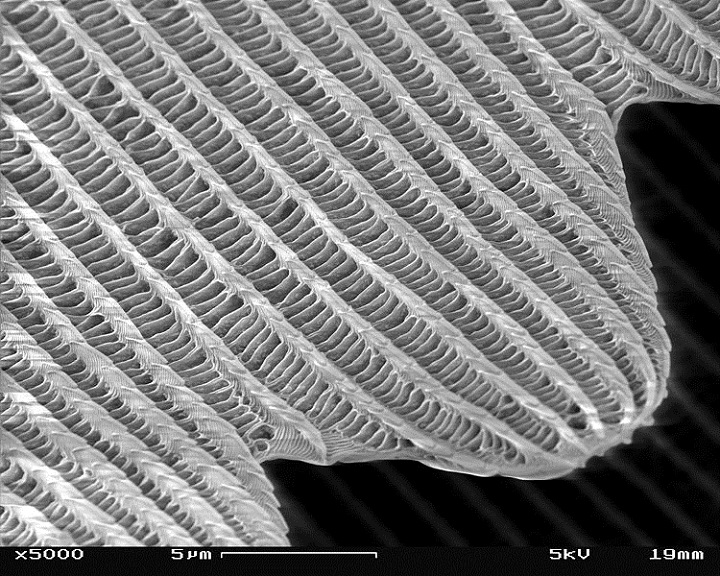
\includegraphics[width=\textwidth]{chapter_1/butterfly3}
		\caption{Magnification 5000x}
		\label{fig:b5000}
	\end{subfigure}
	\caption{Peacock butterfly wing surface using Scanning Electron Microscopy.  Images from wikimedia.org}
	\label{fig:butterfly}
\end{figure}

The work of \cite{lang2011Butterfly} the authors study the effect of such porous structure in the flight performance of butterflies.
Using cameras to measure the kinematics of their flight, they can compute their efficiency to "climb" (generate lift) and the stroke amplitude and frequency.
The authors conclude, after the proper statistical tests on the overall butterfly population, that the porous structure of their wing gives a boost in climbing efficiency about $30\%$; that results clearly stress out the importance of the poroelastic layer of the wings. 
Even though the flight aerodynamic is extremely complex \cite{srygley2002unconventional}, it seems clear that the peculiar structure of the wings surface is critical for their aerodynamic performances.


Superhydrophobic surfaces works as they were water repellent, in fact over such surfaces the water can slide over with much less resistance resulting in very small values of wettability.
This behavior is caused by the microscopic structure that forms the surface \ref{fig:lotus}, in fact the rugosities are arranged in a more or less regular way in order to be able to capture air pockets that rest inside this structures.
These air inclusion provoke an effective slip at the air-liquid interface that cause the drag reduction; but they also change the contact angle of droplets 
The work of \citet{bottaro2003effect} summarize the above aspect and their applications.

\begin{figure}[h]
	\centering
	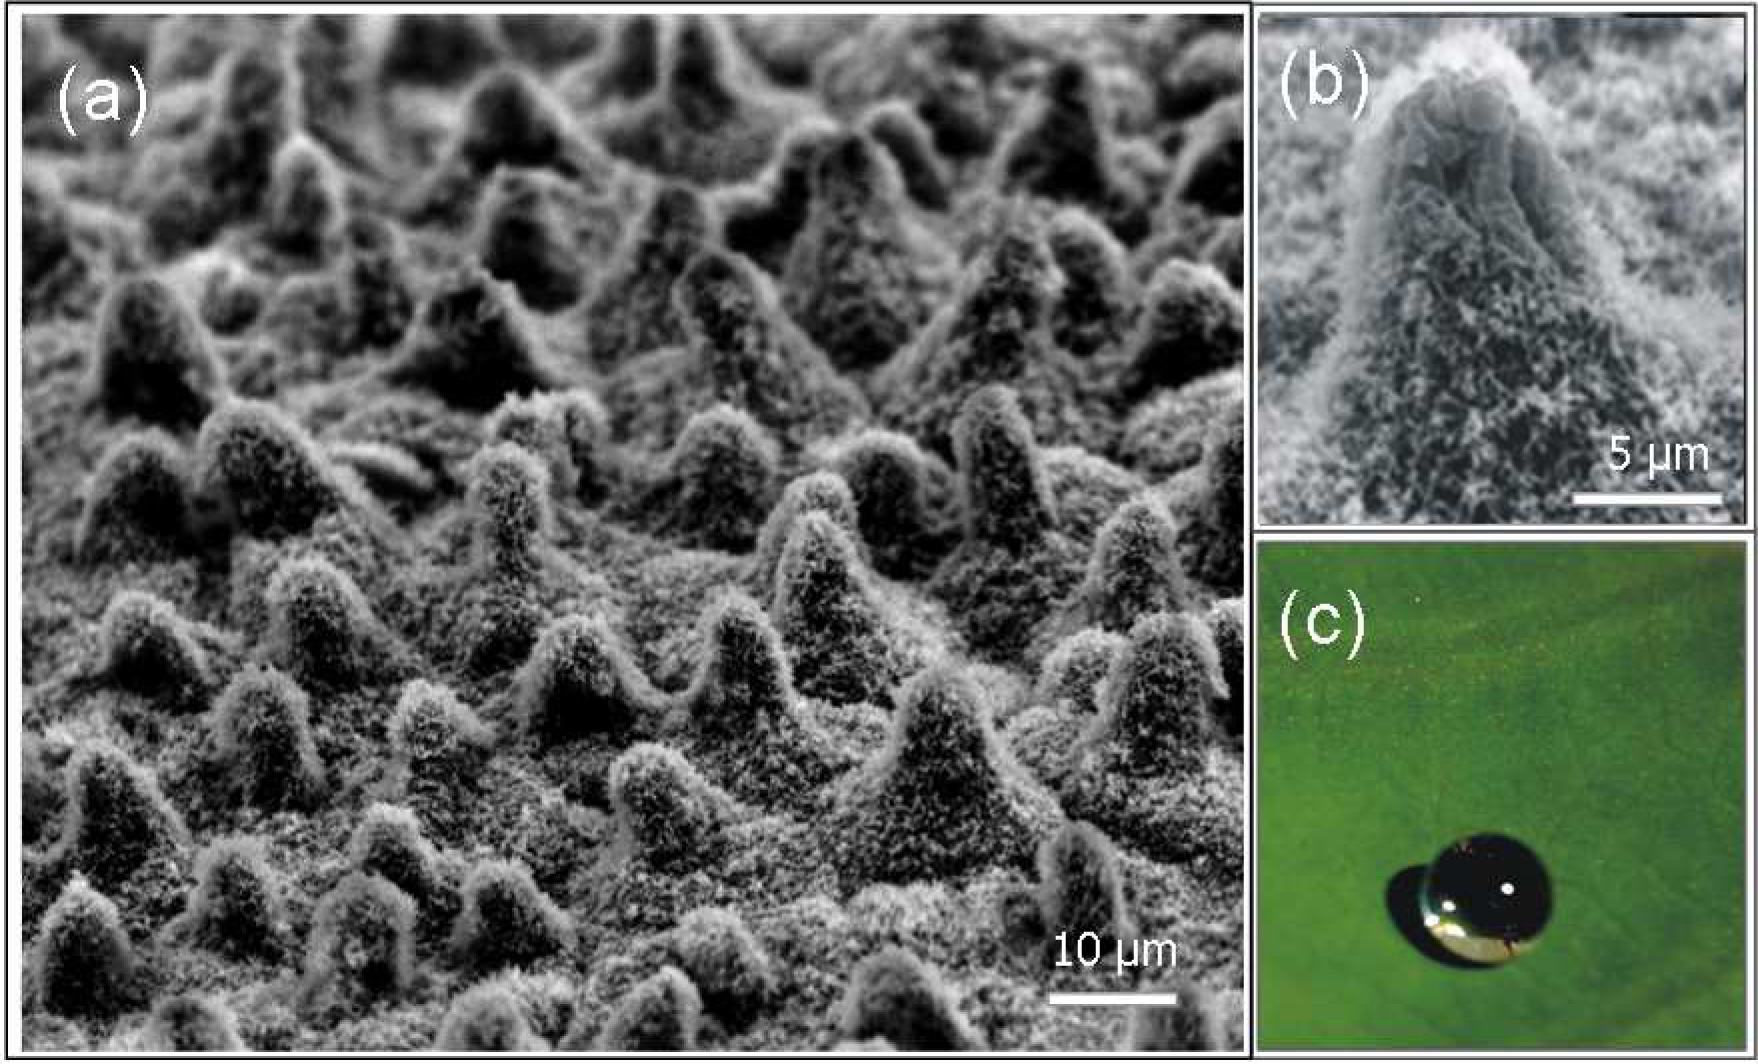
\includegraphics[width=0.6\linewidth]{chapter_1/lotus}
	\caption{(a) Scanning electron microscopy (SEM) image showing the structure of lotus leaf, (b) higher order of magnification on the single protuberance forming the surface and (c) a water drop that due to the contact angle attain an almost spherical shape. Images from \cite{stratakis2009laser}}
	\label{fig:lotus}
\end{figure}


The interest reader could find other examples and broaden the above key aspect also in \cite{bhushan2016biomimetics}, \cite{tropea2012nature}.



\subsection{Riblets and shark-skin surfaces}

We have seen that natural surface can be an inspiration to find some strategies for many aerodynamic problems; in the following we will focus especially on the drag reduction.

Is known that the total drag contribution can be separated in different components, and the classical decomposition is between skin-friction and pressure drag.

Since most of the industrial application involves turbulent flow, obviously there is a lot of research developing solution to reduce the skin-friction in this regime.
Table 6.3.1 in the book of \citet{mclean2012understanding} make a wide list of technique already been proposed on the problem.

As the same author pinpoint the most effective, and probably the most practicable concept, are the riblets.
They are regularly arranged alternating ridges aligned in the streamwise flow direction as the figure \ref{fig:riblets1} show.

\begin{figure}[h]
	\centering
	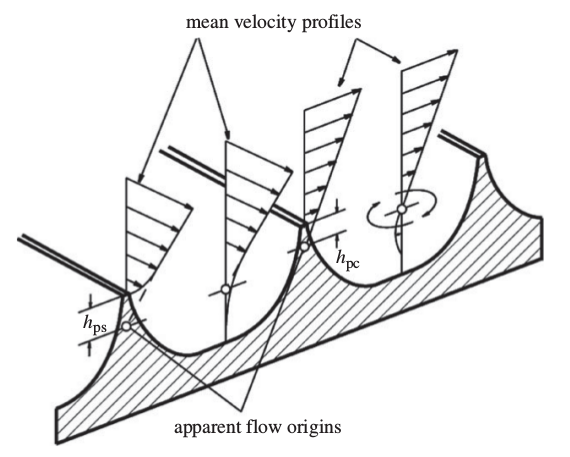
\includegraphics[width=0.7\linewidth]{chapter_1/riblets3}
	\caption{Schematics of the physics ... \citet{bechert1997experiments}}
	\label{fig:riblets1}
\end{figure}

The reduce the skin-friction drag reduction correlates with the spacing between the ridges expressed in wall units $ s^+ $, the typical shape is depicted in \ref{fig:riblets_perf} where the vertical axis show the drag reduction computed against the smooth surface case against the $ s^+ $.
This general shape of the curve, in which the skin friction decrease in certain range of spacing and then increase as the $ s^+ $ increase, is caused by a competition between the capacity of riblets to obstruct lateral fluid flow and an increase in the penetration of high speed vorticies inside this manufactured rugosities.

\begin{figure}[h]
	\centering
	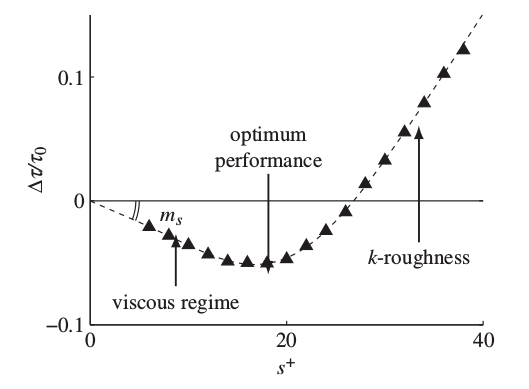
\includegraphics[width=0.7\linewidth]{chapter_1/riblets_performance}
	\caption{Performance ... \citet{jimenez2001turbulent} }
	\label{fig:riblets_perf}
\end{figure}

This last physical explanation of the riblets performances is presented in the schematics \ref{fig:riblets_schem} 


\begin{figure}[h]
	\centering
	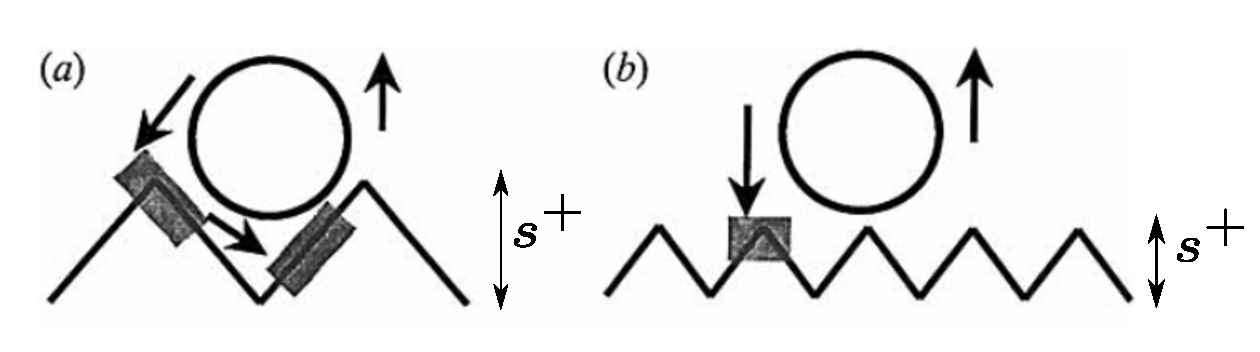
\includegraphics[width=0.7\linewidth]{chapter_1/riblets1}
	\caption{ ... \citet{choi1993direct} }
	\label{fig:riblets_schem}
\end{figure}



Computing the performance of such surfaces can be expensive since the only quantitative theory in such problems are DNS simulations or experiments.
The slope of the curve \ref{fig:riblets_perf} can be predicted by linear stability theory or by means of empirical correlations as in \citet{garcia2011hydrodynamic}

They are robust off-design, forgiving about yaw effect and riblets shape

cita il paper con i riblets nel becco 

Riblets e shark per skin friction

The hulls of the USA challengers in the America’s Cup 1987 and 2010 sailing competitions were fitted with riblets

Luchini 2011 genrating slip delta u+ and offset delta h+

Porous surface(mortazvi) per viscous pressure drag, (pressure redistribution)



\citet{itoh2006turbulent} and \citet{bechert1997experiments} shows that compliant wall can outperform riblets.

\citet{boomsma2016direct} dice che il drag cresce ma è perche usa IBM che con le forze nn ci azzecca, e la superficie nn è elastica



\subsection{Permeable surfaces}

More vertical extended porous surfaces instead try to act on the pressure drag contribution, that depends on the overall pressure distribution on the body.
Usually the pressure contribution is the most significant and even in highly streamlined body its around the $10\%$ of the total drag.

Compliant, surfaces that deflect in response to the surface pressure fluctuation of the boundary layer

cita esperimenti tedeschi sul cilindro con il bordo d'uscita poroso

